\chapter*{Аннотация}		% Заголовок
\addcontentsline{toc}{chapter}{Аннотация}	% Добавляем его в оглавление

В ходе работы разработаны методы работы с графами в системе {\tt Coq}, а также методы работы с правильными раскрасками графов. Реализованы некоторые графы, представленные в статье A. de Grey, <<The chromatic number of the plane is at least 5>>~\cite{deGrey}, а также формализованы и доказаны в системе {\tt Coq} утверждения о типах возможных правильных раскрасок графов
{\tt T} и {\tt H}. Полный код работы расположен по адресу \href{https://github.com/LenaAn/deGrey_proofs}{https://github.com/LenaAn/deGrey\_proofs}.

\chapter*{Введение}		% Заголовок
\addcontentsline{toc}{chapter}{Введение}	% Добавляем его в оглавление

\section{Хроматическое число плоскости. Задача Нелсона — Эрдёша — Хадвигера}

Граф $G$ -- это упорядоченная пара $G := (V, E)$, где $V$ -- конечное непустое множество, а $E$ — подмножество $V\times V$. Если $(u, v) \in E$, то вершины $u$ и $v$ называются { \it смежными}. Обозначение $u \sim v$.

Раскраска $f$ графа $G$ -- это отображение из $V$ в множество цветов. 
Раскраска $f$ называется {\it правильной}, если для любых двух смежных вершин $u$ и $v$ $f(u) \neq f(v)$

{\it Хроматическое число} графа --- это минимальное количество цветов, в которые можно правильно раскрасить граф.

{\it Граф единичных расстояний} -- это граф, вершинами которого являются некоторые точки евклидовой плоскости, а ребрами соединены все пары вершин, находящиеся на расстоянии $1$.

{\it Хроматическое число плоскости $\chi$ } --- это минимальное число цветов $\chi$, в которое можно правильно раскрасить любой граф единичных расстояний.

\begin{figure}[ht] 
  \center
  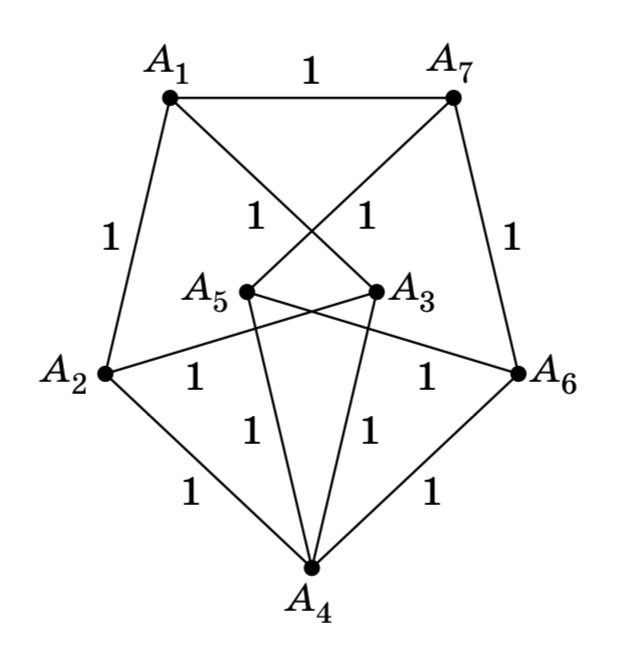
\includegraphics [width=0.5\linewidth] {Moser_Spindle}
  \caption{Веретено Мозера} 
  \label{img:Moser_Spindle}
\end{figure}

Задача Нелсона — Эрдёша — Хадвигера заключается в нахождении хроматического числа плоскости. С 1950 года известно \cite{Soi}, что хроматическое число плоскости не менее 4 и не больше 7. 

\begin{figure}[ht] 
  \center
  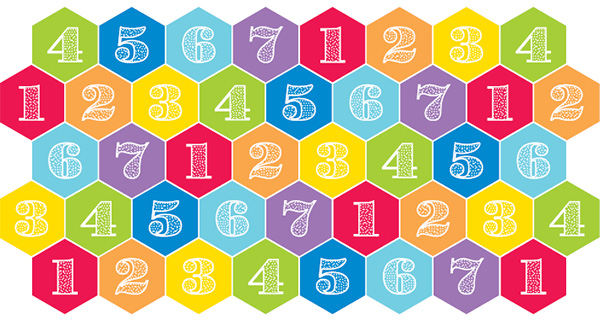
\includegraphics [width=0.8\linewidth] {raskraska7}
  \caption{Раскраска плоскости в 7 цветов} 
  \label{img:raskraska7}
\end{figure}

На рисунке \ref{img:Moser_Spindle} приведен пример графа, который не красится в $3$ цвета, а на рисунке \ref{img:raskraska7} приведено замощение плоскости в $7$ цветов так, что никакая пара точек на расстоянии $1$ не окрашена в один цвет.

В апреле 2018 года Обри де Грей опубликовал статью~\cite{deGrey}, в которой доказал, что хроматическое число плоскости не менее $5$. На момент написания работы задача является открытой.

Целью работы является эффективная формализация конструкций
графов, уточнение, формализация и верификация утверждений статьи в
системе {\tt Coq}.

\section{Система Coq. Описание, история, возможности, применения}
{\tt Coq} -- это компьютерная система
формального представления математических утверждений, алгоритмов и
доказательств. Система обеспечивает интерактивную разработку
гарантированно корректных доказательств, позволяет частично
автоматизировать поиск вывода и содержит достаточно богатую стандартную
библиотеку верифицированных теорем. {\tt Coq} включает в себя развитый язык
функционального программирования и средства автоматического извлечения
программ на языках {\tt ML} и {\tt Haskell}. 

Примеры использования системы:
\begin{itemize}
    \item 
    {\it CompCert}: оптимизирующий компилятор для почти всего языка программирования {\it C}, который полностью формализован и верифицирован на {\tt Coq}.
    \item Структура данных с несвязным множеством: доказательство корректности в {\tt Coq} было опубликовано в 2007 году.
    \item Теорема Фейта – Томпсона: формальное доказательство с использованием {\tt Coq} было завершено в сентябре 2012 года.
    \item Теорема о четырех цветах: формальное доказательство с использованием {\tt Coq} было завершено в 2005 году.
\end{itemize}

\newcommand{\actuality}{}

%% регистрируем счётчики в системе totcounter
\regtotcounter{totalcount@figure}
\regtotcounter{totalcount@table}       % Если поставить в преамбуле то ошибка в числе таблиц
\regtotcounter{TotPages}               % Если поставить в преамбуле то ошибка в числе страниц

% \textbf{Объем и структура работы.} Работа состоит из~введения, трёх глав, заключения и~двух приложений.
%% на случай ошибок оставляю исходный кусок на месте, закомментированным
%Полный объём диссертации составляет  \ref*{TotPages}~страницу с~\totalfigures{}~рисунками и~\totaltables{}~таблицами. Список литературы содержит \total{citenum}~наименований.
%
% Полный объём работы составляет \formbytotal{TotPages}{страниц}{у}{ы}{} 
% с~\formbytotal{totalcount@figure}{рисунк}{ом}{ами}{ами}
% и~\formbytotal{totalcount@table}{таблиц}{ей}{ами}{ами}. Список литературы содержит  
% \formbytotal{citenum}{наименован}{ие}{ия}{ий}.
